

% \documentclass[12pt]{article}
\documentclass[10.8pt, a4paper, USenglish, twocolumn]{article}

\usepackage{isaks_template} % Contains all included packages. See isaks_template.sty.

% latex margins
% \linespread{1.5}
\newgeometry{vmargin={15mm}, hmargin={25mm,37mm}}
%
\title{ {\Large \textbf{Mathematical modelling of cell membranes }} }
% IF ONE AUTHOR
%\address{Norwegian University of Science and Technology \\
%Department of Mathematical Sciences \\
%{\tt isakhammer@gmail.com}}
%

\author{Isak Hammer\footnote{isakhammer@gmail.com} \\{\small Supervisor: André Massing\footnote{Department of Mathematical Sciences, NTNU}} }
\date{\today}
\begin{document}

% Comment this out to remove todos
% https://tex.stackexchange.com/questions/4830/how-to-hide-todo-notes-without-deleting-them-manually
%\renewcommand{\todo}[1]{}
\maketitle
\begin{sloppy}
\textit{ \textbf{Note.} This article is submitted as an examination in the course TK8115 Numerical Optimal Control for the autumn semester 2022 at the Department of Engineering Cybernetics, NTNU. So it is by no means peer-reviewed or validated.}


\begin{abstract}
This article aims to show the latest methods of mathematical modelling of biological cell membranes. We first presented general research on incorporating multi-physics into mathematical models. We then presented a mathematical and numerical shape optimization framework using a gradient flow method and a finite element method to solve cell membrane dynamics specifically for the elastic bending energy on evolving surfaces.
\end{abstract}

    \section{Introduction}


\begin{frame}{Introducing Myself}
    \begin{columns}
        % Column 1
        \begin{column}{0.5\textwidth}
            \begin{itemize}
                \item Isak Hammer, 27 year old, Lofoten
                \item Graduate student in Industrial Mathematics
                \item Research Focus: Numerical methods for Partial Differential Equations (PDEs).
            \end{itemize}
        \end{column}

        % Column 2
        \begin{column}{0.5\textwidth}
            \begin{figure}
                \centering
                \includegraphics[width=0.7\textwidth]{figures/isak.jpg}
            \end{figure}
        \end{column}
    \end{columns}
\end{frame}

\begin{frame}{Importance and Motivation of the Cahn Hilliard Equation}
    \begin{columns}
        % Column 1
        \begin{column}{0.5\textwidth}
            \begin{itemize}
                \item Thermodynamically modelling of a two-component liquid separation\footnotemark[1].
            \item Modelling of so-called lipid rafts in biological membrane dynamics \footnotemark[2].
            \end{itemize}
        \end{column}
        \begin{column}{0.5\textwidth}
            \begin{itemize}
                \item Droplet dynamics, i.e., coalescence, breakup and movement by coupling with Navier-Stokes \footnotemark[3].
            \end{itemize}
        \end{column}
    \end{columns}
    \footnotetext[1]{\fullcite{cahn1959free}}
    \footnotetext[2]{\fullcite{yushutin2019computational}}
    \footnotetext[3]{\fullcite{zimmermann2019calculation}}
\end{frame}

\begin{frame}
    \begin{block}{The Cahn Hilliard Equation}
        The general Cahn Hilliard Equation  has the form $u( x, t): \Omega \times [0,T] \mapsto [-1,1]   $ s.t.
            \[
            \begin{split}
                 u_t+\Delta\left(\varepsilon \Delta u-\frac{1}{\varepsilon} f(u)\right)&=0 \quad \text{in } \Omega \\
\partial_n u=\partial_n \Delta u& =0 \quad \text{on } \Gamma  \\
 u & =u_0 \quad \text{on } \Omega
            \end{split}
            \]
where $f(s)=F^{\prime}(s)$ and $F(s)=\frac{1}{4}\left(s^2-1\right)^2$ and $\Omega \subset \mathbf{R}^d, d=2,3$, is a bounded domain.
\end{block}

\begin{block}{Challenges}
    \begin{enumerate}
        \item Highly nonlinear and stiff. Often practical applications require $\varepsilon \ll 1$.
        \item 4th order system.
        % \item Conservation of mass and the Neumann conditions conditions.
    \end{enumerate}
\end{block}

\end{frame}

\begin{frame}
    \begin{block}{Why Finite Element Method (FEM)}
        \begin{enumerate}
            \item \textbf{Robust mathematical framework}
            \item \textbf{Can easily handle complex geometries}
            \item \textbf{High flexibility of basis functions}
            \item \textbf{Other: } Supports adaptive refinements, easily adaptable to multi-physics problems ++ .
        \end{enumerate}
    \end{block}
\end{frame}

% \begin{frame}
%     \begin{block}{Strategy to solve the Cahn-Hilliard problem on smooth domains}
%         \begin{enumerate}
%             \item Solve the biharmonic problem $\Delta ^2 u = f$ for polygonal domains.
%             \item Modify the method to handle smooth domains.
%             \item Utilize the time integration to handle non-linearity.
%         \end{enumerate}
%     \end{block}
% \end{frame}

% \begin{frame}
%     \begin{block}{Strategy to solve the Cahn-Hilliard problem on smooth domains}
%         \begin{enumerate}
%             \item First find a suitable method to solve an 4th order PDE for polygonal domains.
%             \item Modify the problem formulation to take account for smooth domains.
%             \item Utilize the time integration to handle nonlinearity.
% \item \textcolor{red}{Make the time-steps small enough or implement adaptivity time schemes.}
%         \end{enumerate}
%     \end{block}
% \end{frame}


% \begin{frame}
% \begin{columns}
% \column{0.55\textwidth}
% \begin{block}{The Biharmonic Problem}
% Let $\Omega \subseteq \mathbb{R} ^d$ be a bounded domain with boundary $\Gamma $ . Let the biharmonic problem have the form s.t. $u:\Omega \mapsto \mathbb{R} $,
% \begin{equation}
% \label{eq:bi_problem}
% \begin{split}
% \Delta^2 u + \alpha u & = f( x) \quad \text{in } \Omega, \\
% \partial_{n} u & = g_{1} \quad \text{on } \Gamma , \\
% \partial_{n} \Delta u & = g_{2} \quad \text{on } \Gamma . \\
% \end{split}
% \end{equation}
% Here is $\Delta ^2 = \Delta \left( \Delta \right) $ the biharmonic operator. The functions $g_{1},g_{2}: \Omega \to \mathbb{R}$ are denoted as boundary conditions.
% \end{block}

% \column{0.45\textwidth}
% \begin{figure}[htpb!]
%     \centering
%     \begin{tikzpicture}
%         % Circle
%         \draw (0.0,0.0) circle (1.5cm);
%         \fill[blue!30] (0.0,0.0) circle (1.5cm);

%         \draw[->, line width=1.0pt] ({1.5*cos(65)}, { 1.5*sin(65) }) -- ({ 2.5*cos(65)  }, { 2.5*sin(65)  }) node[ above left] {$n $};
%         % \draw[->, line width=1.0pt] ({1.5*cos(45)}, { 1.5*sin(45) }) -- ({ 1.5*cos(45) - 1.5*sin(45) }, { 1.5*sin(45) + 1.5*cos(45) }) node[ above right] {$t $};

%         % Labels
%         \node[below right] at (0.5,0.5) {$\Omega$};
%         \node[below right] at (-1.5,-1.2) {$\Gamma$};
%     \end{tikzpicture}
%     \caption{ Illustration of the domain $\Omega $, the boundary $\Gamma $ and the normal vector $n$. }
%     \label{fig:domain_construction}
% \end{figure}
% \end{columns}

% \end{frame}

\begin{frame}
    \frametitle{The Biharmonic Problem (on a polygon)}
    \begin{columns}
        \column{0.55\textwidth}
        \begin{block}{}
            Let $\Omega \approx \Omega_{h} = \mathcal{T}_{h}$ be a bounded \textcolor{red}{polygonal} domain with boundary $\Gamma $ . Let the biharmonic problem have the form s.t. $u:\Omega \mapsto \mathbb{R} $,
            \begin{equation}
                \label{eq:bi_problem}
                \begin{split}
                    \Delta^2 u + \alpha u & = f( x) \quad \text{in } \Omega, \\
                    \partial_{n} u & = 0 \quad \text{on } \Gamma , \\
                    \partial_{n} \Delta u & = 0 \quad \text{on } \Gamma . \\
                \end{split}
            \end{equation}
            Here is $\Delta ^2 = \Delta \left( \Delta \right) $ the biharmonic operator.
        \end{block}

        \column{0.45\textwidth}
        \begin{figure}[htpb!]
            \centering
            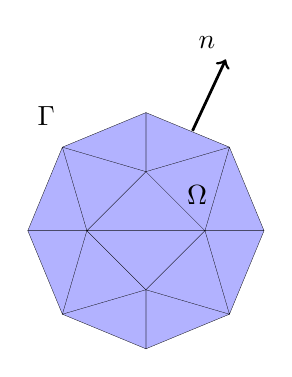
\begin{tikzpicture}
                % FIGURE OF FITTED MESH
                % Boundary points
                \foreach \i in {0, 45, ..., 315} {
                    \coordinate (boundary-\i) at (\i:1.5cm);
                }
                % Interior points
                \coordinate (interior-1) at (0.75, 0);
                \coordinate (interior-2) at (-0.75, 0);
                \coordinate (interior-3) at (0, 0.75);
                \coordinate (interior-4) at (0, -0.75);

                % Create a cycle connecting all the boundary points
                \fill[blue!30] (boundary-0) -- (boundary-45) -- (boundary-90) -- (boundary-135) -- (boundary-180) -- (boundary-225) -- (boundary-270) -- (boundary-315) -- cycle;

                % Labels
                \node[below right] at (0.4,0.7) {$\Omega $};
                \node[below right] at (-1.5,1.7) {$\Gamma $};

                % Triangulation (manually specified)
                \draw[line width=0.1pt] (boundary-0) -- (boundary-45) -- (interior-1) -- cycle;
                \draw[line width=0.1pt] (boundary-45) -- (boundary-90) -- (interior-3) -- cycle;
                \draw[line width=0.1pt] (boundary-90) -- (boundary-135) -- (interior-3) -- cycle;
                \draw[line width=0.1pt] (boundary-135) -- (boundary-180) -- (interior-2) -- cycle;
                \draw[line width=0.1pt] (boundary-180) -- (boundary-225) -- (interior-2) -- cycle;
                \draw[line width=0.1pt] (boundary-225) -- (boundary-270) -- (interior-4) -- cycle;
                \draw[line width=0.1pt] (boundary-270) -- (boundary-315) -- (interior-4) -- cycle;
                \draw[line width=0.1pt] (boundary-315) -- (boundary-0) -- (interior-1) -- cycle;

                % Triangulation between interior points
                \draw[line width=0.1pt] (interior-1) -- (interior-2) -- (interior-3) -- cycle;
                \draw[line width=0.1pt] (interior-1) -- (interior-2) -- (interior-4) -- cycle;

                \draw[->, line width=1.0pt] ({1.4*cos(65)}, { 1.4*sin(65) }) -- ({ 2.4*cos(65)  }, { 2.4*sin(65)  }) node[ above left] {$n $};

            \end{tikzpicture}
            \caption{ Illustration of the mesh $\Omega_{h} $, the boundary $\Gamma $ and the normal vector $n$. }
            \label{fig:domain_construction}
        \end{figure}
    \end{columns}
\end{frame}



\begin{frame}
\frametitle{ $C^0$ Interior Penalty Method (CIP) for the Biharmonic Problem }

\begin{block}{}
The proposed numerical scheme is to find an  $w \in V_{h}$ .t.
\begin{equation*}
\label{eq:CP_A_F}
a_{h}( w, v )   = l_{h}( v) = ( f,v)_{\Omega } , \quad \forall v \in V_{h}  .
\end{equation*}
where
\begin{equation*}
\begin{split}
a_{h} \left( w, v \right)   =&
    \left( \alpha  w, v \right) _{\Omega }   +  \left( \Delta  w, \Delta v \right) _{\Omega } \\
 & +
  \left( \mean{  \Delta  w }, \jump{ \partial _{n }v} \right)_{\mathcal{F}_{h}}  +
 \left( \mean{ \Delta  v }, \jump{ \partial _{n}w }      \right)_{\mathcal{F}_{h}}  + \frac{\gamma }{h}  \left( \jump{ \partial _{n} w}, \jump{ \partial _{n} v   }   \right)_{\mathcal{F}_{h}}
 % l_{h}( v_{h}) & =  \left( f, v \right) _{\Omega }
\end{split}
\end{equation*}

Which is inspired from Brenner2012 \footnotemark[1]
\end{block}

\footnotetext[1]{\fullcite{brenner2012}}

\end{frame}


\begin{frame}
\frametitle{Cut Finite Element Method (CutFEM)}

\begin{block}{Unfitted mesh vs fitted mesh}
    CutFEM is a numerical method for solving partial differential equations (PDEs) using an unfitted mesh.

\begin{figure}
    \centering
    % First TikZ picture
    \begin{minipage}{0.45\textwidth}
        \centering
        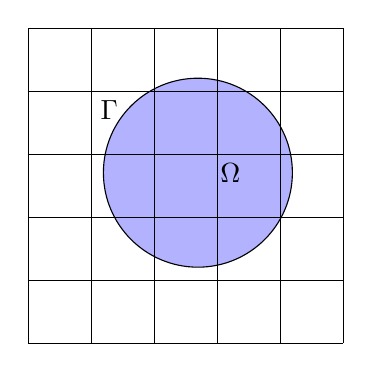
\begin{tikzpicture}[scale=0.80]
            \draw[fill=blue!30] (0.2, 0.2) circle (1.5cm);
            % Background mesh
            \foreach \i in {-2.5, -1.5, ..., 2.5} {
                \draw[line width=0.1pt, shift={(-2.5,\i)}] (0,0) -- (5,0);
                \draw[line width=0.1pt, shift={(\i,-2.5)}] (0,0) -- (0,5);
            }
            % Labels
            \node[below right] at (0.4,0.5) {$\Omega $};
            \node[below right] at (-1.5,1.5) {$\Gamma $};
            % \draw[blue, thick] (-2.5, -2.5) rectangle (2.5, 2.5);
        \end{tikzpicture}
    \end{minipage}
    \hfill
    % Second TikZ picture
    \begin{minipage}{0.45\textwidth}
        \centering
        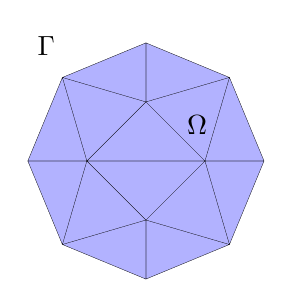
\begin{tikzpicture}[scale=1.0]
            % FIGURE OF UNFITTED MESH
            % Boundary points
            \foreach \i in {0, 45, ..., 315} {
                \coordinate (boundary-\i) at (\i:1.5cm);
            }
            % Interior points
            \coordinate (interior-1) at (0.75, 0);
            \coordinate (interior-2) at (-0.75, 0);
            \coordinate (interior-3) at (0, 0.75);
            \coordinate (interior-4) at (0, -0.75);

            % Create a cycle connecting all the boundary points
            \fill[blue!30] (boundary-0) -- (boundary-45) -- (boundary-90) -- (boundary-135) -- (boundary-180) -- (boundary-225) -- (boundary-270) -- (boundary-315) -- cycle;

            % Labels
            \node[below right] at (0.4,0.7) {$\Omega $};
            \node[below right] at (-1.5,1.7) {$\Gamma $};

            % Triangulation (manually specified)
            \draw[line width=0.1pt] (boundary-0) -- (boundary-45) -- (interior-1) -- cycle;
            \draw[line width=0.1pt] (boundary-45) -- (boundary-90) -- (interior-3) -- cycle;
            \draw[line width=0.1pt] (boundary-90) -- (boundary-135) -- (interior-3) -- cycle;
            \draw[line width=0.1pt] (boundary-135) -- (boundary-180) -- (interior-2) -- cycle;
            \draw[line width=0.1pt] (boundary-180) -- (boundary-225) -- (interior-2) -- cycle;
            \draw[line width=0.1pt] (boundary-225) -- (boundary-270) -- (interior-4) -- cycle;
            \draw[line width=0.1pt] (boundary-270) -- (boundary-315) -- (interior-4) -- cycle;
            \draw[line width=0.1pt] (boundary-315) -- (boundary-0) -- (interior-1) -- cycle;

            % Triangulation between interior points
            \draw[line width=0.1pt] (interior-1) -- (interior-2) -- (interior-3) -- cycle;
            \draw[line width=0.1pt] (interior-1) -- (interior-2) -- (interior-4) -- cycle;

            % \draw[blue, thick] (-2.5, -2.5) rectangle (2.5, 2.5);

        \end{tikzpicture}
    \end{minipage}


    % \caption{Mesh comparison: unfitted mesh (left) adheres to domain and boundary, while fitted mesh (right) employs a triangular mesh for polygonal approximation of the circular domain.}
    \label{fig:domain_mesh}
    \end{figure}
\end{block}

\end{frame}

\begin{frame}
    \frametitle{Cut Finite Element Method}
Background Mesh
    \begin{block}{}
        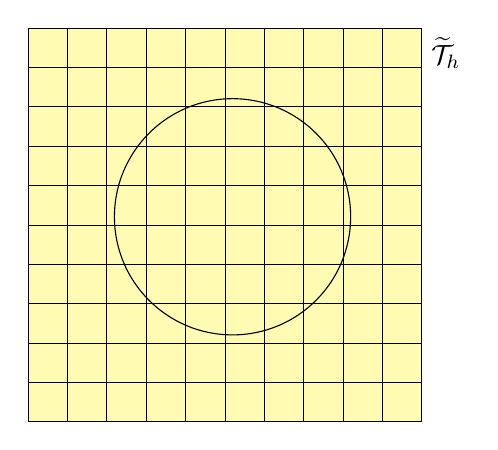
\begin{tikzpicture}[scale=1.0]

            \fill[yellow!30] (-2.5,2.5) -- (2.5,2.5) -- (2.5,-2.5) -- (-2.5,-2.5) -- cycle;

            \draw (0.1, 0.1) circle (1.5cm);
            % Background mesh
            \foreach \i in {-2.5, -2, ..., 2.5} {
                \draw[line width=0.1pt, shift={(-2.5,\i)}] (0,0) -- (5,0);
                \draw[line width=0.1pt, shift={(\i,-2.5)}] (0,0) -- (0,5);
            }


            % Labels
            \node[below right] at (2.5,2.5) {$\widetilde{\mathcal{T}}_{h}$};
        \end{tikzpicture}
    \end{block}
\end{frame}

\begin{frame}
    \frametitle{Cut Finite Element Method}
    Active Mesh
    \begin{block}{}
        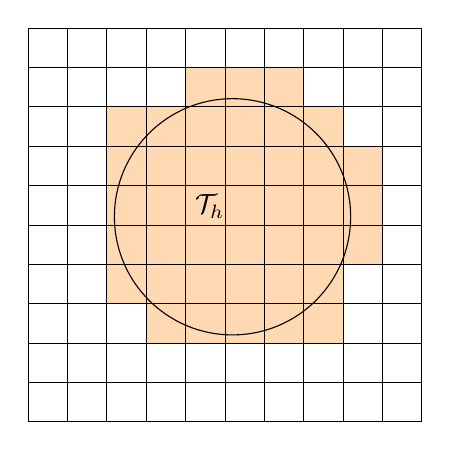
\begin{tikzpicture}[scale=1.0]

            % POTENTIAL ACTIVE MESH
            \fill[orange!30] (2,2) -- (2,-1.5) --(-1.5,-1.5) -- (-1.5,2) -- cycle;

            % ELEMENTS WITH NO INTERSECTION
            % lower left
            \fill[white] (-1.5,-1.5) rectangle (-1.0,-1.0);
            \fill[white] (-1.5,2.0) rectangle (-1.0,1.5);
            \fill[white] (-1.0,2.0) rectangle (-0.5,1.5);
            \fill[white] (2,2) rectangle (1.5,1.5);
            \fill[white] (1.5,2) rectangle (1.0,1.5);
            \fill[white] (2,1.5) rectangle (1.5,1.0);
            \fill[white] (1.5,-1) rectangle (2,-1.5);
            \fill[white] (1.5,-0.5) rectangle (2,-1.0);

            % CUT ELEMENTS
            \fill[orange!30] (-0.5,2.0) rectangle (1.0,1.5);
            \fill[orange!30] (-1.5,1.5) rectangle (0.0,1.0);
            \fill[orange!30] (0.5,1.5) rectangle (1.5,1.0);
            \fill[orange!30] (-1.5,1.0) rectangle (-1.0,-1.0);
            \fill[orange!30] (-1.0,-0.5) rectangle (-0.5,-1.5);
            \fill[orange!30] (-0.5,-1.5) rectangle (1.5,-1.0);
            \fill[orange!30] (1.5,-1) rectangle (1.0,-0.0);
            \fill[orange!30] (1.5,-0.5) rectangle (2.0,1.0);
            \fill[orange!30] (1.0,0.5) rectangle (1.5,1.0);

            \draw (0.1, 0.1) circle (1.5cm);
            % Background mesh
            \foreach \i in {-2.5, -2, ..., 2.5} {
                \draw[line width=0.1pt, shift={(-2.5,\i)}] (0,0) -- (5,0);
                \draw[line width=0.1pt, shift={(\i,-2.5)}] (0,0) -- (0,5);
            }


            % Labels
            % \node[below right] at (2.5,2.5) {$\widetilde{\mathcal{T}}_{h}$};
            % \node[below right] at (0.4,0.5) {$\mathcal{T}_{int}$};
            \node[below right] at (-0.5,0.5) {$\mathcal{T}_{h }$};
        \end{tikzpicture}
    \end{block}
\end{frame}

\begin{frame}
    \frametitle{Cut Finite Element Method}
    Interior Mesh and Cut Cells
    \begin{block}{}
        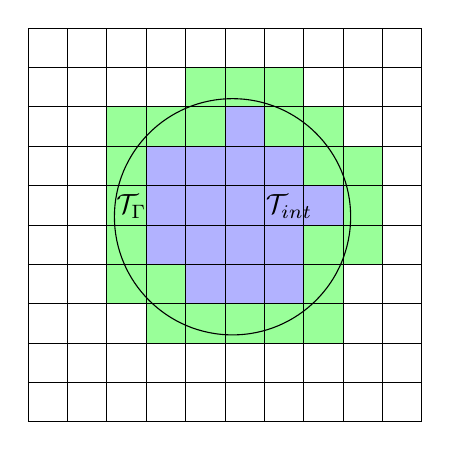
\begin{tikzpicture}[scale=1]

            % POTENTIAL ACTIVE MESH
            \fill[blue!30] (2,2) -- (2,-1.5) --(-1.5,-1.5) -- (-1.5,2) -- cycle;

            % ELEMENTS WITH NO INTERSECTION
            % lower left
            \fill[white] (-1.5,-1.5) rectangle (-1.0,-1.0);
            \fill[white] (-1.5,2.0) rectangle (-1.0,1.5);
            \fill[white] (-1.0,2.0) rectangle (-0.5,1.5);
            \fill[white] (2,2) rectangle (1.5,1.5);
            \fill[white] (1.5,2) rectangle (1.0,1.5);
            \fill[white] (2,1.5) rectangle (1.5,1.0);
            \fill[white] (1.5,-1) rectangle (2,-1.5);
            \fill[white] (1.5,-0.5) rectangle (2,-1.0);

            % CUT ELEMENTS
            \fill[green!40] (-0.5,2.0) rectangle (1.0,1.5);
            \fill[green!40] (-1.5,1.5) rectangle (0.0,1.0);
            \fill[green!40] (0.5,1.5) rectangle (1.5,1.0);
            \fill[green!40] (-1.5,1.0) rectangle (-1.0,-1.0);
            \fill[green!40] (-1.0,-0.5) rectangle (-0.5,-1.5);
            \fill[green!40] (-0.5,-1.5) rectangle (1.5,-1.0);
            \fill[green!40] (1.5,-1) rectangle (1.0,-0.0);
            \fill[green!40] (1.5,-0.5) rectangle (2.0,1.0);
            \fill[green!40] (1.0,0.5) rectangle (1.5,1.0);

            \draw (0.1, 0.1) circle (1.5cm);
            % Background mesh
            \foreach \i in {-2.5, -2, ..., 2.5} {
                \draw[line width=0.1pt, shift={(-2.5,\i)}] (0,0) -- (5,0);
                \draw[line width=0.1pt, shift={(\i,-2.5)}] (0,0) -- (0,5);
            }


            % Labels
            \node[below right] at (0.4,0.5) {$\mathcal{T}_{int}$};
            \node[below right] at (-1.5,0.5) {$\mathcal{T}_{\Gamma }$};
        \end{tikzpicture}
    \end{block}
\end{frame}

\begin{frame}
\frametitle{Cut Finite Element Method (CutFEM)}

A recent and promising numerical technique for PDEs, has gained significant momentum in the past decade \footnotemark[1]\footnotemark[2].

\begin{block}{}
    \begin{itemize}
        \item  Complex domains and moving domains efficiently.
        \item Utilizing so-called ghost penalties to ensure well-posedness.
        % \item Dividing the computational domains into \textbf{background} , \textbf{active}, \textbf{cut}  and \textbf{interior} mesh.
    \end{itemize}
\end{block}
\footnotetext[1]{\fullcite{burman2015cutfem}}
\footnotetext[2]{\fullcite{gurkan2019stabilized}}

\end{frame}




% \begin{frame}
% \frametitle{ Cut $C^0$ Interior penalty method (CutCIP) }

% \begin{block}{}
% The discretized numerical problem is to solve $w \in V_{h}$ such that
% \begin{equation*}
% \label{eq:CP_A_F}
% A( w, v )  = a_{h}( w,v) + \textcolor{red}{g_{h}( w,v)}  = l_{h}( v), \quad \forall v \in V_{h}  .
% \end{equation*}

% Where the additional bilinear term $g_{h}( w,v) : V_{h} \times V_{h} \to  \mathbb{R} $ is the so-called \textbf{ghost penalty}, which does the numerical regularization to ensure stability on cut cells.

% \end{block}

% \end{frame}

\begin{frame}
\frametitle{ CutCIP Method}

My master's thesis is dedicated to demonstrating that the relevant properties remain valid for CutCIP formulation still holds.

    \begin{block}{Well-posedness }
         The discrete bilinear form $a_{h}$ is wellposed on $V_{h}$ if this holds; \[
             \begin{split}
                 (Coercivity) \quad  A( v,v) &  \gtrsim  \| v \|_{A }^{ 2 } \quad  \forall v \in  V_{h} \\
            (Boundedness) \quad A( v,w) & \lesssim  \| v \|_{A }^{  }\| w \|_{a_{h} }^{  } \quad  \forall v,w \in  V_{h}
             \end{split}
        \]
    \end{block}

    \begin{block}{Apriori Estimates }

         Let $u$ be the solution to the strong problem with the corresponding discrete solution $u_{h}$ with polynomical order $k\ge 2$ .
        Then does it exist  $l = \min_{} ( 2, k)  $ s.t.
\[
        \| u - u_{h} \|_{a_{h}  }^{  } \lesssim  h^{l-1} \| u \|_{ H^{l} ( \Omega ) }^{  }
\]
    \end{block}
    % \footnotetext[1]{\fullcite{Gu2012}}
\end{frame}



\begin{frame}
\frametitle{ Cut $C^0$ Interior Penalty Method (CutCIP) Results }
% \frametitle{Manufactured Solution}


\begin{block}{Manufactured solution}
    In the experiments will we only consider polynomial order $k=2$.
We consider the manufactured solution:
$$
u_{ex}(\mathbf{x}) = \left(x_1^2 + x_2^2 - 1\right)^2 \cos(2\pi x_1) \cos(2\pi x_2)
$$
where $\mathbf{x}=(x_1,x_2)$ and $\Omega=\{(x_1,x_2): x_1^2 + x_2^2 \le  1\}$.
This manufactured solution can be used to test the accuracy of numerical methods for solving the above differential equation.
\end{block}
\end{frame}


\begin{frame}
\frametitle{ Cut $C^0$ Interior penalty method (CutCIP) Results }
\resizebox{\textwidth}{!}{
\begin{tabular}{rrrrrrrrr}
    \hline\hline
    \textbf{$n$} & \textbf{$\Vert e \Vert_{L^2}$} & \textbf{EOC} & \textbf{$ \Vert e \Vert_{H^1}$} & \textbf{EOC} & \textbf{$\Vert e \Vert_{ a_h,* }$} & \textbf{EOC} & \textbf{Cond number} & \textbf{ndofs} \\\hline
    4 & 2.4E+00 &  & 3.3E+00 &  & 6.2E+01 &  & 8.7E+04 & 8.1E+01 \\
    8 & 3.6E-01 & 2.72 & 1.1E+00 & 1.60 & 3.9E+01 & 0.68 & 5.1E+05 & 2.4E+02 \\
    16 & 2.2E-02 & 4.06 & 2.5E-01 & 2.12 & 1.4E+01 & 1.51 & 3.7E+06 & 8.3E+02 \\
    32 & 5.6E-03 & 1.97 & 6.0E-02 & 2.04 & 3.6E+00 & 1.93 & 2.8E+07 & 3.0E+03 \\
    64 & 1.4E-03 & 2.00 & 1.5E-02 & 2.02 & 9.2E-01 & 1.96 & 2.1E+08 & 1.1E+04 \\
    128 & 3.5E-04 & 2.00 & 3.7E-03 & 2.01 & 2.4E-01 & 1.94 & 1.7E+09 & 4.3E+04 \\\hline\hline
  \end{tabular}
}
\end{frame}






\begin{frame}
\frametitle{ Cut $C^0$ Interior penalty method (CutCIP) Results }

\begin{figure}[h!]
    \centering
    \resizebox{0.6\textwidth}{!}{% Recommended preamble:
% \usetikzlibrary{arrows.meta}
% \usetikzlibrary{backgrounds}
% \usepgfplotslibrary{patchplots}
% \usepgfplotslibrary{fillbetween}
% \pgfplotsset{%
%     layers/standard/.define layer set={%
%         background,axis background,axis grid,axis ticks,axis lines,axis tick labels,pre main,main,axis descriptions,axis foreground%
%     }{
%         grid style={/pgfplots/on layer=axis grid},%
%         tick style={/pgfplots/on layer=axis ticks},%
%         axis line style={/pgfplots/on layer=axis lines},%
%         label style={/pgfplots/on layer=axis descriptions},%
%         legend style={/pgfplots/on layer=axis descriptions},%
%         title style={/pgfplots/on layer=axis descriptions},%
%         colorbar style={/pgfplots/on layer=axis descriptions},%
%         ticklabel style={/pgfplots/on layer=axis tick labels},%
%         axis background@ style={/pgfplots/on layer=axis background},%
%         3d box foreground style={/pgfplots/on layer=axis foreground},%
%     },
% }

\begin{tikzpicture}[/tikz/background rectangle/.style={fill={rgb,1:red,1.0;green,1.0;blue,1.0}, fill opacity={1.0}, draw opacity={1.0}}, show background rectangle]
\begin{axis}[point meta max={nan}, point meta min={nan}, legend cell align={left}, legend columns={1}, title={}, title style={at={{(0.5,1)}}, anchor={south}, font={{\fontsize{14 pt}{18.2 pt}\selectfont}}, color={rgb,1:red,0.0;green,0.0;blue,0.0}, draw opacity={1.0}, rotate={0.0}, align={center}}, legend style={color={rgb,1:red,0.0;green,0.0;blue,0.0}, draw opacity={1.0}, line width={1}, solid, fill={rgb,1:red,1.0;green,1.0;blue,1.0}, fill opacity={1.0}, text opacity={1.0}, font={{\fontsize{8 pt}{10.4 pt}\selectfont}}, text={rgb,1:red,0.0;green,0.0;blue,0.0}, cells={anchor={center}}, at={(1.02, 1)}, anchor={north west}}, axis background/.style={fill={rgb,1:red,1.0;green,1.0;blue,1.0}, opacity={1.0}}, anchor={north west}, xshift={1.0mm}, yshift={-1.0mm}, width={94.6mm}, height={74.2mm}, scaled x ticks={false}, xlabel={$\delta$}, x tick style={color={rgb,1:red,0.0;green,0.0;blue,0.0}, opacity={1.0}}, x tick label style={color={rgb,1:red,0.0;green,0.0;blue,0.0}, opacity={1.0}, rotate={0}}, xlabel style={at={(ticklabel cs:0.5)}, anchor=near ticklabel, at={{(ticklabel cs:0.5)}}, anchor={near ticklabel}, font={{\fontsize{11 pt}{14.3 pt}\selectfont}}, color={rgb,1:red,0.0;green,0.0;blue,0.0}, draw opacity={1.0}, rotate={0.0}}, xmajorgrids={true}, xmin={-0.001471665988344504}, xmax={0.05052719893316125}, xticklabels={{$0.00$,$0.01$,$0.02$,$0.03$,$0.04$,$0.05$}}, xtick={{0.0,0.010000000000000002,0.020000000000000004,0.030000000000000006,0.04000000000000001,0.05000000000000001}}, xtick align={inside}, xticklabel style={font={{\fontsize{8 pt}{10.4 pt}\selectfont}}, color={rgb,1:red,0.0;green,0.0;blue,0.0}, draw opacity={1.0}, rotate={0.0}}, x grid style={color={rgb,1:red,0.0;green,0.0;blue,0.0}, draw opacity={0.1}, line width={0.5}, solid}, axis x line*={left}, x axis line style={color={rgb,1:red,0.0;green,0.0;blue,0.0}, draw opacity={1.0}, line width={1}, solid}, scaled y ticks={false}, ylabel={$\kappa(A)$}, y tick style={color={rgb,1:red,0.0;green,0.0;blue,0.0}, opacity={1.0}}, y tick label style={color={rgb,1:red,0.0;green,0.0;blue,0.0}, opacity={1.0}, rotate={0}}, ylabel style={at={(ticklabel cs:0.5)}, anchor=near ticklabel, at={{(ticklabel cs:0.5)}}, anchor={near ticklabel}, font={{\fontsize{11 pt}{14.3 pt}\selectfont}}, color={rgb,1:red,0.0;green,0.0;blue,0.0}, draw opacity={1.0}, rotate={0.0}}, ymode={log}, log basis y={10}, ymajorgrids={true}, ymin={100000.0}, ymax={1.0e25}, yticklabels={{$10^{5}$,$10^{10}$,$10^{15}$,$10^{20}$,$10^{25}$}}, ytick={{100000.0,1.0e10,1.0e15,1.0e20,1.0e25}}, ytick align={inside}, yticklabel style={font={{\fontsize{8 pt}{10.4 pt}\selectfont}}, color={rgb,1:red,0.0;green,0.0;blue,0.0}, draw opacity={1.0}, rotate={0.0}}, y grid style={color={rgb,1:red,0.0;green,0.0;blue,0.0}, draw opacity={0.1}, line width={0.5}, solid}, axis y line*={left}, y axis line style={color={rgb,1:red,0.0;green,0.0;blue,0.0}, draw opacity={1.0}, line width={1}, solid}, colorbar={false}]
    [\addlegendimage{empty legend}] \addlegendentry[font={{\fontsize{11 pt}{14.3 pt}\selectfont}}, text={rgb,1:red,0.0;green,0.0;blue,0.0}] {\hspace{-.6cm}{\textbf{$(\gamma, \gamma_1, \gamma_2)$}}}
    \addplot[color={rgb,1:red,0.0;green,0.0;blue,1.0}, name path={e73f70a5-bbbd-4a24-8407-eef9d08bc09d}, draw opacity={1.0}, line width={1}, solid]
        table[row sep={\\}]
        {
            \\
            0.0  1.2679164207221107e8  \\
            0.012263883236204186  1.2718633484176141e8  \\
            0.024527766472408372  1.2693944128424127e8  \\
            0.03679164970861256  1.2718633338545807e8  \\
            0.049055532944816745  1.2679164340263365e8  \\
        }
        ;
    \addlegendentry { $1.0 \cdot 10^{1}$, $0.5 \cdot 10^{1}$, $1.0 \cdot 10^{-1}$ }
    \addplot[color={rgb,1:red,1.0;green,0.0;blue,0.0}, name path={8dbacc37-3690-4b1f-9d5d-1b6f1fc900ac}, draw opacity={1.0}, line width={1}, solid]
        table[row sep={\\}]
        {
            \\
            0.0  4.639960110962716e10  \\
            0.012263883236204186  4.932252358128007e12  \\
            0.024527766472408372  4.0959531093983247e12  \\
            0.03679164970861256  4.932252223523245e12  \\
            0.049055532944816745  4.639960117645048e10  \\
        }
        ;
    \addlegendentry { $1.0 \cdot 10^{1}$, $ 0.0 \cdot 10^{0} $, $ 0.0 \cdot 10^{0} $ }
\end{axis}
\end{tikzpicture}
}
    \caption{The plot presents the $L^2$ and $H^1$ error norms and the error in the energy norm ($\Vert e \Vert_{a_h,*}$).}
    \label{fig:CutFEM_error1}
\end{figure}

\end{frame}

\begin{frame}
\frametitle{The Cahn Hilliard Equation}
    \begin{columns}
        % Left column
        \begin{column}{0.5\textwidth}
            \begin{block}{Recall}
                The problem has the form $u( x, t): \Omega \times [0,T] \mapsto [-1,1]$ s.t.
                \[
                \begin{split}
                    u_t+\Delta\left(\varepsilon \Delta u-\frac{1}{\varepsilon} f(u)\right)&=0 \quad \text{in } \Omega \\
                    \partial_n u=\partial_n \Delta u& =0 \quad \text{on } \Gamma  \\
                    u & =u_0 \quad \text{on } \Omega
                \end{split}
                \]
                where $f(u)$ is a nonlinear function.
            \end{block}
        \end{column}
        % Right column
        \begin{column}{0.5\textwidth}
            \begin{block}{Plan forward}
                \begin{enumerate}
                    \item We have now a tool to solve the $\Delta ( \Delta u) $ operator
                    \item Will utilize the time-iteration scheme to solve non-linearity
                \end{enumerate}
            \end{block}
        \end{column}
    \end{columns}
\end{frame}


\begin{frame}
\frametitle{The CutCIP Cahn-Hilliard Formulation}


Drawing upon the concepts delineated in Feng\footnotemark[1], the most efficient approach to address the nonlinear term is by employing an implicit-explicit (IMEX) scheme.

\begin{block}{IMEX method on the CutCIP formulation}
    Let $u^{m}_{h} \in V_{h}$ for the timesteps $m=0,1,\ldots,M$. Let $u_{h}^{0} = u_{0}$ be the initial timestep, then is.
\[
(\overline{\partial}  _{t} u_{h}^m, v_h ) + \varepsilon A (u_{h}^{m}, v_h )+\frac{1}{\varepsilon} c_h ( u_{h}^{m-1}, v_h)=0 \quad \forall v_h \in V_h^m .
\]
Here is $c_{h}( . , .) $ an the nonlinear terms handled in a implicit fashion. The $ \overline{\partial}  _{t}$ operator is simply a finite difference scheme in time-dimension.

\end{block}

\footnotetext[1]{\fullcite{feng2007fully}}
\end{frame}

\begin{frame}
\frametitle{The CutCIP Cahn-Hilliard Experiments}
Implemented using the Gridap FEM framework written in Julia \footnotemark[1].


\begin{block}{Simulation parameters}
    \begin{itemize}
        \item Physical domain $\Omega$  is a 4 discs of radius $R=1$ with distance $d=0.999$, i.e. they are touching!
        \item Inital data is $u_0 = random(-1,1)$ in physical domain $\Omega $.
        % \item Backgroundmesh with size ($L\times L$ ) for $L=2$ and $n=128$.
        % \item Polynomial order $k=2$ .
        % \item Physical parameter $\varepsilon  = \frac{1}{30}$.
        % \item Time-step $\tau = \varepsilon ^{2} \frac{1}{10} $ for the interval $ 0\le t \le 10^3 \tau $.
    \end{itemize}
\end{block}

\footnotetext[1]{\fullcite{badia2020gridap}}


\end{frame}

\begin{frame}
\frametitle{The CutCIP Cahn-Hilliard Experiments}

\begin{figure}[h]
    \centering
    \includegraphics[width=0.5\textwidth]{CH-example/0.png}
    \caption{Iteration 0}
    \label{fig:your_image_label}
\end{figure}
\end{frame}

\begin{frame}
\frametitle{The CutCIP Cahn-Hilliard Experiments}

\begin{figure}[h]
    \centering
    \includegraphics[width=0.5\textwidth]{CH-example/1.png}
    \caption{Iteration 1}
\end{figure}
\end{frame}

\begin{frame}
\frametitle{The CutCIP Cahn-Hilliard Experiments}
\begin{figure}[h]
    \centering
    \includegraphics[width=0.5\textwidth]{CH-example/10.png}
    \caption{Iteration 10}
\end{figure}
\end{frame}

\begin{frame}
\frametitle{The CutCIP Cahn-Hilliard Experiments}
\begin{figure}[h]
    \centering
    \includegraphics[width=0.5\textwidth]{CH-example/50.png}
    \caption{Iteration 50}
\end{figure}
\end{frame}

\begin{frame}
\frametitle{The CutCIP Cahn-Hilliard Experiments}
\begin{figure}[h]
    \centering
    \includegraphics[width=0.5\textwidth]{CH-example/200.png}
    \caption{Iteration 200}
\end{figure}
\end{frame}

\begin{frame}
\frametitle{The CutCIP Cahn-Hilliard Experiments}
\begin{figure}[h]
    \centering
    \includegraphics[width=0.5\textwidth]{CH-example/1000.png}
    \caption{Iteration 1000}
\end{figure}
\end{frame}


\begin{frame}
\frametitle{Further work}
\begin{enumerate}
    \item Adaptive time steps.
    \item Further numerical validation.
    \item Extend the method to handle moving domains.

\end{enumerate}
\end{frame}


\begin{frame}
\frametitle{Questions?}
\end{frame}



    

\section{Background Theory}%
\label{sec:differential_geometry}


\subsection{Differential Calculus}%
\label{sub:differential_calculus}

This subsection is inspired by the notation used in \cite{kovacs2021convergent, dougan2012first}.
Let some initial surface $\Gamma^{0} \subset \mathbb{R} ^3  $ smooth compact and oriented surface with no boundary where we can assign a unique point $p \in \Gamma ^{0}$. We define define the time evolutionary surface to be on the form,
\[
    \begin{split}
\Gamma  = \Gamma \left( t \right) & = \Gamma \left( \chi \left( p,t \right)  \right) \\
                                  &= \left\{ \chi \left( p,t \right): \ p \in \Gamma^{0}  \right\}
    \end{split}
\]
transformed via the smooth mapping,
\[
\chi : \Gamma^{0} \times  \left[ 0,T \right]  \mapsto  \mathbb{R} ^3.
\]
An important regularity result is that if $\Gamma ^{0}$ is of class $C^{\infty}$, then $\Gamma $ is also of class $C^{\infty}$ for $\forall t \in \left[ 0,T \right] $ \cite{sokolowski1992introduction, dougan2012first}.
\todo[inline]{ Formally in \cite[p 48]{sokolowski1992introduction}, it might be an idea to formulate normal unit-vector regularity as $C^{\infty}$ }

We will define a unique evolutionary point $x \in \Gamma \left( t \right) $ based on the smooth mapping $\chi \left( p,t \right) = x$. A way to imagine this is to have a initial point in $\Gamma ^{0}$ and the mapping $\chi $ describes how this point will deform over time. The outer unit normal vector field of $\Gamma \left( t \right) $ is defined as the mapping $\nu : \Gamma \mapsto
\mathbb{R} ^{3}$.

Using the notation presented in \cite{dougan2012first} and \cite{kovacs2021convergent} can we define the basic surface differential operators. Consider a scalar function, $u: \Gamma \mapsto \mathbb{R} $, and a vector-valued function, $\hat{u}: \Gamma  \mapsto \mathbb{R} ^3$. We can then denote $ \nabla _{\Gamma } u: \Gamma \mapsto \mathbb{R} ^{3}$ as the tangential operator,
$$
\nabla_{\Gamma
} u  = \nabla u - \left<\nu, \nabla u \right> \nu.
$$
Similarly, for the vector-valued function is the operator defined s.t.
$$\nabla_{\Gamma } \hat{u} = \left( \nabla_{\Gamma } u_{1},\nabla_{\Gamma } u_{2},\nabla_{\Gamma } u_{3}   \right)^{T}.$$ The surface divergence for a vector-valued function is defined as \[
\nabla_{\Gamma } \cdot \hat{u} = \nabla  \cdot \hat{u} - \nu^{T} D \hat{u} \cdot \nu
\]
Here $D\hat{u}$ denotes the Jacobian of $\hat{u}$. Similarly, the Laplace-Beltrami operator $\Delta _{\Gamma }u: \Gamma \mapsto \mathbb{R}$ is defined s.t.
\begin{equation*}
    \begin{split}
 \Delta _{\Gamma } u  & = \nabla _{\Gamma } \cdot  \nabla _{\Gamma }u \\
 &=  \Delta u  - \nu ^{T} D^2 u \cdot \nu - H \partial _{\nu } f
    \end{split}
.\end{equation*}
Here is $D^2u$ denotes as the Hessian of the scalar function $u$. In the case of a vector valued function is the operator defined as \[
\Delta _{\Gamma } \hat{u} = \left( \Delta _{\Gamma } u_{1}, \Delta _{\Gamma } u_{2}, \Delta _{\Gamma } u_{3} \right)^{T}
\]
A method to compute the mean curvature and the so-called Frobenius norm of matrix $A$ involves applying the
extended Weingarten map, $ A\left( x \right) = \nabla \nu \left( x \right) $, s.t. these identities holds \cite{kovacs2021convergent},
\begin{equation*}
    \begin{split}
    H & = tr(A) = k_{1} + k_{2} \\
    \left\lvert A \right\rvert^{2}  & = k_{1}^2 + k_{2}^2
    \end{split}
.\end{equation*}


\subsection{Evolutionary Surface Dynamics}%
\label{sub:evolutionary_equations}

In this section will we develop a framework evolutionary surface dynamics.

First of all, we can denote the velocity field $v: \Gamma \mapsto \mathbb{R} ^3$ to be
\begin{equation}
    \label{eq:vel}
\frac{dx }{ d t}  = v\left( x \right) \quad \forall x \in \Gamma \left( t \right) .
.\end{equation}
Given a model of the velocity $v$ can we solve the ordinary differential equation (ODE) \eqref{eq:vel} and determine the evolution of a point on the surface $\Gamma\left( t \right)  $.

% Define shape derivatives
Recall that the point $x = \chi \left( p,t \right)  $ is arising from the smooth mapping from the point $p $ in  $\Gamma ^{0} $ to $\Gamma \left( t \right) $. Now, let some arbitrary energy functional have the form,
\[
\mathcal{J} = \int_{\Gamma }^{} \varphi \left( x, \Gamma^{0}  \right) .
\]
For instance, in the case presented in \eqref{eq:WE} we define $\varphi = H ^2$. Based on \cite{dougan2012first},the shape derivative of this energy functional at some time $t$ in the direction of the velocity-field $v$ from \eqref{eq:vel} is defined as \[
d \mathcal{J} \left( \Gamma \left( t \right) ; v  \right) = \lim_{\varepsilon  \to 0} \frac{\mathcal{J} \left( \Gamma \left( t + \varepsilon  \right) - \mathcal{J}\left( \Gamma \left( t  \right) \right)      \right)}{\varepsilon }.
\]

Assume we have a scalar function $f: \Gamma\left( t \right)  \mapsto \mathbb{R}  $. Similarly, as for the shape derivative, we can now denote the material derivative at time $t$ as
\[
    \begin{split}
\frac{D}{Dt}  f\left( x,t \right)  & = \frac{d}{dt} f \left( \chi \left( p,t \right) , t \right) \\
&= \lim_{\varepsilon \to 0}  \frac{f \left( \chi \left( p, t + \varepsilon  \right)  \right) - f \left( \chi \left( p, t  \right)  \right) }{ \varepsilon }
    \end{split}
\]



% Using the definition from \cite{bonito2010parametric, troltzsch2010optimal} can we define the shape derivative of some energy
% functional $\mathcal{J} \left( \Gamma \left( t \right)  \right)  $ towards any directions $ w \forall w \in \mathcal{V}  $  to be the limit

% % Det e no som skurra i dennar notasjonen
% \begin{equation*}
%     \begin{split}
% d\mathcal{J} \left( \Gamma \left( t \right) ; w  \right)  & = \lim_{t \to 0} \frac{\mathcal{J}\left( \Gamma \left( t \right)  \right) - \mathcal{J} (  \Gamma \left( 0 \right))}{t} \\
% &= \left(  \varphi ,w\right)_{\Gamma \left( t \right) }  \\
%     \end{split}
% .\end{equation*}
% \todo[inline]{ Dennar definisjonen e litt rar, sjekk Troltzsch ch2.6 istedenfor  } The notation used here is $\left( v,w \right)_{\Gamma } = \int_{\Gamma }^{}  vw   $ for some $ v,w \in L^{2}\left( \Gamma \right) $ .

% Our goal is to develop the evolutionary dynamics by minimizing the energy functional \eqref{eq:WE}.

% To minimize our energy functional \eqref{eq:WE} of the surface dynamics will we utilize a method called gradient flows. Gradient flows in surface partial differential equation (PDE) are used to solve physical problems where the surface is changing due to some external force. The PDE describes how the surface changes over time in response to this force, thus allowing us to model real-world phenomena such as fluid and heat flow. The gradient of the surface PDE determines the direction and magnitude of the change over time, while the PDE itself may contain additional terms that modify or influence the solution. \cite{dogan2007discrete} An alternative approach would be to solve the problem using standard shape optimization techniques using $\Gamma$ as a variable surface \cite{dalphin2014study}.
% We say that the $L^{2}$  gradient flow is defined as
% \[
% \left( \dot{\chi } , w \right)_{\Gamma \left( t \right)  } = -d\mathcal{J}\left( \Gamma \left( t \right); w  \right).
% \]





    

\newpage
\section{The Willmore flow}%
\label{sec:evolutionary_pde_s_of_the_willmore_flow}



\begin{lemma}
The shape derivative of\eqref{eq:WE} has the form
\[
    \begin{split}
        d\mathcal{E} \left( \Gamma; w  \right)  =& \int_{\Gamma \left( t \right) }^{}  \nabla_{\Gamma } H  \nabla _{\Gamma } w    \\
    & - \int_{\Gamma }^{} H  |\nabla _{\Gamma }  w |^{2} w   \\
    &  + \frac{1}{2} \int_{\Gamma }^{} H^{3} w
    \end{split}
\]

\end{lemma}

\begin{proof}
    Proof can be found in \cite{willmore1996riemannian}
\end{proof}






    
\section{Numerical Methods}%
\label{sec:numerical_methods}


 To be able to find a numerical approximation the weak formulation \eqref{eq:WE_weak_form} will we to formulate a evolving surface element method (ESFEM) for the evolutionary equation PDE's coupled with the evolving surface velocity. We will mostly
 use the notation and methods described in \cite{kovacs2021convergent, hu2022evolving}.

\subsection{ Triangular mesh for $\Gamma ^{0}$  }%
\label{sub:triangular_mesh}

Let initial surface $\Gamma ^{0} \in  \mathbb{R} ^3$ have the triangular mesh $\mathcal{T}_{h} $ constisting of triangles $T$. We will assume that the mesh is inform, i.e., for any $T_{1}, T_{2}$ $T_{1} \neq T_{2}$ and $T_{1} \cap T_{2} \neq \emptyset
$, then must $T_{1}$  and $T_{2}$ share either a vertex or a facet. Let diameter of each triangle $h_{T}$  be denoted as,
\[
    \begin{split}
    h_{T} & = \max_{x_{1}, x_{2} \in \Gamma ^{0}} dist(x_{1}, x_{2}), \\
h_{min} & = \min_{T \in \mathcal{T} _{h}} h_{T}, \\
h_{max} & = \max_{T \in \mathcal{T} _{h}} h_{T},
    \end{split}
\]
where $h_{min}$ and $h_{max}$ is the maximum and minimum diameter of an individual triangle $T$ in $\mathcal{T}_{h} $. We define the chunkiness parameter $c_{T} = h_{T}/r_{T}$, where $r_{T}$ is the largest ball inside inscribed in $T$. We will then
assume that the mesh is shape regular and quasi-uniform, i.e., $c_{T} \le c $ and $h_{max} \le c h_{min} $ for a  constant $c$ independent of $h_{T} $ and $T$.
For more information, see \cite{dziuk2007finite}.
\todo[inline]{  Apparently some quasi-uniform and shape regular definitions in \cite{dziuk2007finite}, need to check this.}

\subsection{Surface element method}%
\label{sub:surface_element_method}
In this section is the goal to develop discrete analogs of the definitions we introduced in subsections \ref{sub:differential_calculus} and \ref{sub:evolutionary_equations}.


Let $\mathcal{T}_{h}  $ be the triangulation of $\Gamma ^{0}$. Now denote the vector $ \mathbf{x} = \mathbf{x} \left( t \right)  \in \mathbb{R} ^{3N}$ as a collection of all evolving nodes, $x_{j}\left( t \right)  \in  \mathbb{R} ^3$, $j = \mathcal{I} $, by a piecewise polynomial interpolation
with degree $k$. Here is the index of all the nodes defined as $\mathcal{I} =\left\{ 1, \ldots, N \right\}  $, where $N$ is the total number of nodes.

We denote the discretized surface, $\Gamma _{h} \left[ \mathbf{x}\left( t \right)  \right] $, to be the numerical approximation of the surface $\Gamma \left( t \right) $. As an initial condition do we construct the initial nodes, $
 x_{j}( 0 )  = p_{j} \forall j \in  \mathcal{I}  $, s.t.
 $\Gamma _{h}^{0  } = \Gamma _{h} \left[ \mathbf{x}\left( 0 \right)   \right] $ interpolates the initial surface, $\Gamma ^{0}$ in the nodal points $p_{j} \in \Gamma ^{0}, \  j \in  \mathcal{I} $.

An essential piece of the puzzle is the finite element basis on $\Gamma _{h}\left[ \mathbf{x} \right] $ which is denoted to have the form,
\[
 \phi_{j} \left[ \mathbf{x} \right]: \Gamma_{h}\left[ \mathbf{x} \right] \mapsto \mathbb{R} , \quad   j \in  \mathcal{I} .
\]
\todo[inline]{ How can the basis vectors move? And how is it related to the definition of $X_{h}$ later in the subsection?  }
In fact, the basis satisfies the identity, \[
\phi _{j} \left[ \mathbf{x} \right] \left( x_{i} \right)  = \delta _{ij} \quad \forall i,j \in  \mathcal{I} .
\]

Finally, we can now define the so-called evolving finite element space of $\Gamma _{h}\left[ \mathbf{x}\left( t \right)  \right] $ as, \[
    \begin{split}
S_{h}\left[ \mathbf{x} \right]   & = S_{h}\left( \Gamma _{h}\left[ \mathbf{x} \right]  \right) \\
 & = span\left\{ \sum_{j \in  \mathcal{I}  }^{}  c_{j} \phi _{j}\left[ \mathbf{x} \right]  \mid  c_{j} \in \mathbb{R}   \right\}.
    \end{split}
\]

The discretized surface mapping, $X_{h}: \Gamma_{h} ^{0} \mapsto  \Gamma _{h} \left[ \mathbf{x}\left( t \right)  \right] $, is denoted as \[
X_{h}\left( p_{h},t \right) = \sum_{j \in \mathcal{I} }^{}  x_{j}\left( t \right)  \phi \left[ x\left( 0 \right)  \right] \left( p_{h} \right), \  p_{h} \in \Gamma ^{0}_{h},
\]
and the problem obviously does satisfy the identities; $X_{h}\left( p_{h},0 \right)  = p_{h} \forall p_{h} \in \Gamma _{h}$, the evolutionary property $X_{h} \left( p_{j}, t \right)  = x_{j}\left( t \right)  \forall j \in \mathcal{I} $, and
\[
    \begin{split}
        \Gamma _{h} & = \Gamma_{h} \left( t \right) =   \Gamma_{h} \left[ \mathbf{x}\left( t \right)  \right]  \\
                                    &= \Gamma_{h}\left[ X_{h}\left( \cdot ,t \right)  \right] \\
&=\left\{ X_{h}\left( p_{h},t \right): p_{h} \in  \Gamma ^{0}_{h} \right\}.
    \end{split}
\]
\todo[inline]{TODO: Need to check if the definition of $\Gamma _{h}\left[ \mathbf{x}  \right] = \Gamma_{h}\left[ X_{h}\left( \cdot ,t \right)  \right] $ makes sense. Also made $\Gamma _{h} = \Gamma _{h}\left[ \mathbf{x}\left( t \right)  \right] $ som et kunstig innslag. }
For shorthand notation do we define the discretized point as $x_{h} = X_{h}\left( p_{h},t \right) \in \Gamma _{h} $.
Thus discretized velocity $v_{h}\left( x_{h},t \right): \Gamma _{h} \mapsto  \mathbb{R} ^{3} $ is defined as \[
    v_{h}\left( x_{h},t \right)  = \sum_{j \in \mathcal{I} }^{} v_{j}\left( t \right) \phi _{j}\left[ \mathbf{x}\left( t \right)  \right] \left( x_{h} \right)
\]
Hence, the evolutionary discrete velocity is defined as $ \frac{d}{dt}x_{h} = v_{h}\left( x_{h},t \right).$















    \section{Conclusion}

We have presented several interesting multiphysics processes to consider when modelling cell membrane dynamics. First, we introduced an elastic bending energy on evolving surfaces using the Canham-Helrich energy functional \eqref{eq:CH} and the equivalent Willmore energy functional. Secondly, we established that the diffusion of a two-phase system can be modelled using the Ginzburg-Landau energy functional \eqref{eq:GL} and discussed how we could combine the energy functional models to do multiphysics problems. 

To demonstrate the techniques used to solve physical problems on evolving domains, we chose the Willmore energy functional \eqref{eq:WE}. The background theory of calculus on surfaces and evolutionary dynamics was briefly discussed and then applied to define the strong and weak (or integral) formulation of the system dynamics. We then established a basic numerical framework and introduced the evolution surface finite element method.


    \printbibliography
\end{sloppy}

\end{document}
